\documentclass{article}
\usepackage{fullpage}
\usepackage[utf8]{inputenc}
\usepackage[title]{appendix}
\usepackage{amsmath}
\usepackage{amssymb}
\usepackage{amsthm}
\usepackage{url}
\usepackage{graphicx}
\graphicspath{ {./images/} }

\newcommand{\figref}[1]{Figure \ref{#1}}
\newcommand{\tabref}[1]{Table \ref{#1}}
\newcommand{\apdxref}[1]{Appendix \ref{#1}}

\newcommand{\CH}{\mathrm{CH}}

\title{Minimum Perimeter-Sum Bipartition Implementation}
\author{Allen Mi, Haakon Flatval}
\date{December 2018}

\begin{document}

\maketitle

\begin{abstract}
    The Minimum Perimeter-Sum Bipartition problem is stated as follows: Given set of points in the Euclidean plane, partition it into two subsets such that the sum of perimeters of their convex hulls is as small as possible. In this text, we describe our implementation of the algorithm by Abrahamsen et al \cite{abb17} and provide analyses on its behaviour given different inputs.
    % Fill in more here / rewrite abstract as things happen
\end{abstract}

\section{Introduction}
The Minimum Perimeter-Sum Bipartition problem is the problem of partitioning a set of points in the two-dimensional plane into two disjoint subsets $P_1$ and $P_2$ such that the sum of the perimeters of $\text{CH}(P_1)$ and $\text{CH}(P_2)$ is minimized, where $\text{CH}(P)$ is the convex hull of the set of points $P$. In 2017, Abrahamsen et al \cite{abb17} devised an algorithm that solves this problem in time $O(n \log^4 n)$, $n$ being the number of points in the input. 

% Fill out more details about bounds and related work - like in the algorithmic paper?
\subsection{The Scope of this Project}

Our goal has been to assess the effects of various inputs on the running time of an implementation of the algorithm \cite{abb17}. 

We have not implemented the entire algorithm, but has concentrated on the subroutines we have identified to impose the greatest impact on the running time. 
We have failed to implement one of the important subroutines - the one we call \texttt{combine\_convex\_hulls} - within time bound. We have not been able to identify a way that allows us to withhold this bound in practice. We will discuss this issue by the end of this report.

In addition to implementing a number of the subroutines, we give here an analysis of how different input sets affect the performance of the algorithm, and discuss our method of constructing such input sets.

Our implementation is publicly available \cite{hm18}.

\section{Background}

% Description of the problem and the algorithm

Abrahamsen et al. \cite{abb17} shows that, for any optimal partition $\{P_1^*, P_2^*\}$ of the input points, the following holds:

\textit{Either the outer angle between the inner tangents of the convex hulls
$\text{CH}(P_1^*)$ and $\text{CH}(P_2^*)$ (see illustration) is at least $\pi / 6$, or the smallest distance between two
points in $P_1^*$ and $P_2^*$ is at least $1/250 \cdot \min(\text{per}(P_1^*), \text{per}(P_2^*))$}. 

$\text{per}(P)$ denotes the length of the perimeter of the convex hull of $P$. In figure \figref{fig:tangent_angle}, we show the two inner tangents of two polygons $L_1$ and $L_2$ of the polygons, with the outer angle $B$ in-between them.

In the remainder of the discussion, the angle $B$ is referred to as the separation angle.

This immediately splits our approach into two cases, one where we assume the separation angle to be at least $\pi / 6$, and another where we assume the distance between the sets to be "large". 


We solve the problem with each of these assumptions in turn, and choose the best of the results as our answer.


\begin{figure}[ht]
    \centering
    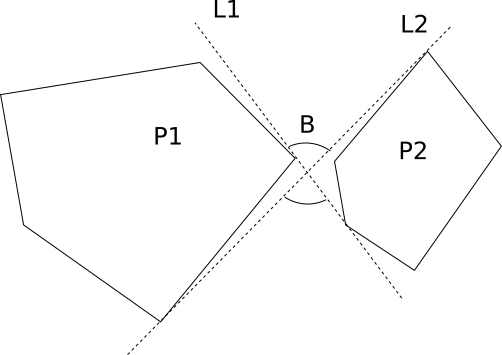
\includegraphics[width=0.5\textwidth]{images/inner_angle.png}
    \caption{The inner tangents $L_1$ and $L_2$ and their outer angle $B$}
    \label{fig:tangent_angle}
\end{figure}


\subsection{Algorithm Assuming Large Separation Angle of Solution}

In the case where the separation angle is larger than $\pi / 6$, we make the following observation: Consider the set of seven angles $\Phi = \{\pi \cdot i / 7 \,  | \, i \in [0, 7) \}$. There must exist a line separating the optimal subsets, whose angle is among those seven. Thus, we will approach as follows:

For each of the angles $\phi \in \Phi$, we use a line $l_\phi$ having angle $\phi$ in a Graham's scan; that is, we treat $l_\phi$ as a scanning line in a modified version of Graham's algorithm: When first scanning from one side to the other, we compute the "upper" hull, as usual, but we also make sure to store the length of the upper hull ending at each intermediate point. The same is done for the the lower hull when scanning the other way, and the process is repeated switching the direction of scan for upper and lower hull. 

Now, each point has four lengths associated with it (from being the end point for the upper and lower hull from each of the two scanning directions), which makes it easy for us to compute the total length of any convex hull ending at each point in constant time. Scanning through the points again, repeatedly using the two points immediately to each side of the scanning line and computing the length two hulls ending at these points, we can find the best possible partition with separating line of angle $\phi$.

Repeating this approach for each of the seven angles, we will, by assumption of large separation angle, find the best partition overall.

This approach uses Graham's algorithm a constant number of times, and thus has a complexity of $O(n \log n)$.

\subsection{Algorithm Assuming Large Separation Distance of Solution}

Now, we must find the best possible partition assuming the distance between the two subsets is large. 

We first treat the special case where one of the subsets is a single point $p$. Some thought reveal that $p$ must lie on the convex hull of the set of input points $P$. We will thus go through each of the points $v_i$ at the boundary of $\text{CH}(P)$ in turn and compute the perimeter $\text{per}(P \setminus \{v_i\}$. 

We do this by constructing each triangle $\Delta_i$ formed by three consecutive points on the boundary $v_{i - 1}$, $v_i$ and $v_{i + 1}$, and find the set $P_i$ of the points contained inside $\Delta_i$, excluding $v_i$, but including $v_{i - 1}$ and $v_{i + 1}$. Note now that each point can belong to a maximum of two triangles. According to $\cite{abb17}$, doing this is "easy" in $O(n \log n)$ time, without specifying how. We have chosen to compute the set $P_i$ in the following way:
\begin{itemize}
    \item Construct a suitable center point $c$ not contained in any triangle \textit{We find this by taking the crossing between two diagonals}
    \item Sort the points by their angle around the center point, such that a chosen first boundary point $v_0$ has angle $0$
    \item Initialize $t_0 = \Delta_0$, $t_1 = \Delta_1$
    \item Iterate over each point $p_i$: \begin{itemize}
        \item If $p_i$ is the end point of $t_0$, shift $t_0$ and $t_1$ to the next $\Delta$
        \item If $p_i$ is inside $t_0$ or $t_1$ (or both), put it in the triangle's respective set
    \end{itemize}
\end{itemize}

Finally, having found the sets $P_i$, we compute the convex hulls $\text{CH}(P_i)$, and can find the perimeters $\text{per}(P \setminus \{v_i\})$ as $\text{per}(P \setminus \{v_i\}) = \text{per}(P) - |v_{i - 1}v_i| - |v_iv_{i + 1}| + \text{per}(P_i) - |v_{i - 1}v_{i + 1}|$.

Thus, finding the optimal partition where one of the sets is a single point, can be done in $O(n \log n)$ time.

Now we have reduced the problem to the following: Partition the set $P$ into two non-trivial sets with smallest sum of perimeters. 

$\cite{abb17}$ proceeds at this point to compute a set $S$ of $O(n)$ axis-aligned squares which is certain to contain a so-called \textit{good} square,  a square in the plane that fully contains one of the optimal subsets, and such that one edge of the square is no larger than 18 times the perimeter of that optimal subset.

We will not go into detail as to how the set $S$ is computed, as the technique uses a compressed quad tree \cite{quad_trees}, which is well beyond what there is place for here given reasonable prerequisites. We also find it unlikely to be a bottleneck for our analysis, which we will discuss later. The algorithm runs in $O(n \log n)$ time. For the remainder of this discussion, we will assume that we have found the set $S$ of squares, among which at least one is \textit{good}.

What we will do in the following, is to intersect each of the $O(n)$ square $\sigma_i$ in $S$ with a constant number of lines $l_j$, each line representing the boundary of a half plane $h_j$. For each such half plane, we will find the set of points within the square, and also within the half plane: $P \cap \sigma_i \cap h_j$. 

From the way we construct these half planes (which we will review shortly), and from the assumption of large separation distance, if $\sigma_i$ is a good square, the set $P \cap \sigma_i \cap h_j$ will be one of the optimal sets for some half plane $h_j$ (Lemma 8 in \cite{abb17}). We will thus compute all such sets in intersections of a half plane and a square, and pick the one optimizing the perimeter lengths. The remainder of this section will assess how we proceed to compute these set intersections and the corresponding perimeter lengths.

The half planes are constructed as follows: $4 \cdot 18 / \dfrac{1}{250} + 1 = 18001$ points are placed evenly around the perimeter of the square. The number is chosen such that the distance between two neighboring points is less than the separation distance between the optimal sets. Now, we create the set of lines connecting every pair of these points. We thus create a set of $O(18001^2)$ lines, which are the boundaries of the half planes $h_j$.

The next question we have to answer, is how to find the set $P \cap \sigma_i \cap h_j$, and also $\text{per}(P \cap \sigma_i \cap h_j)$ fast. Notice that this is a query for a set of points in a rectangular axis-align region, then cut against a half plane. A normal two-level range tree \cite{range_trees} can be used for query for sets contained in axis-align rectangles, and adding one more level for the half plane axis (perpendicular to the half plane boundary) ensures that we can now also easily find a set of points on a specific side of the half plane. 

Thus, for each of the half planes constructed, we also construct a range tree. Now, note that for any square, all the lines we constructed for that square will have its counterpart lines in other squares with the same angle and relative placement within the square. Since the sorting of the lowest level of the range tree will only depend on the angle of the respective half plane, we will only need to construct a constant number of range trees, one for each half plane angle. 

As mentioned, when finding the set $P \cap \sigma_i \cap h_j$ with a range tree query, we are also interested in finding its perimeter. We can do this by augmenting each node of the lowest level trees in the range tree to contain the convex hull of all nodes in the subtree rooted at that node. This can be done recursively, in the sense that the convex hull of a node can be computed by combining the hulls at its two children. We have implemented this by computing the outer tangents (so that the two polygons lie on the same side of each tangent) using \cite{ks95}, and their touch points on both polygons, and tracing the original hulls, but upon hitting a touch point, switches to the corresponding touch point of the other polygon. We remark that \cite{ks95} directly computes the touch point indices in the polygons, and not the tangent lines themselves.

This construction gives us a range tree that contains convex hulls at its nodes in $O(n \log^3 n)$ time and using $O(n \log^3 n)$ space. Now. a general query region of the form $\sigma_i \cap h_j$ will in $O(\log^3n)$ time return $O(\log^3 n)$ nodes from the range tree, each covering a disjoint subset of the points in the query region. We will also make a few more disjoint queries into the range tree, in order to find $P \setminus (\sigma_i \cap h_j)$. We will need up to five more queries of the same form as the first. 

Now we have found a candidate partition, the set of points within $\sigma_i \cap h_j$ and the set of points outside. We have now a collection of $O(\log^3 n)$ convex hulls representing each of the region. In the last part of this section, we show how to compute the combined hull and perimeter length of each of those collections. 

The general approach to combine a set of convex hulls into one, is to scan over them using Graham's scan. We first construct a new set of polygons in the following way: Create two "events" for each polygon, one corresponding to its first (leftmost) point, and the second to its last point (rightmost) point. Sort this list, and traverse it. Imagine this as a scan line scanning over the polygons left to right. We keep track of all the currently "active" polygons in a balanced binary tree (e.g. a red-black tree), sorted on their y-coordinate (which is well defined between "active" polygons, as the they are disjoint). Whenever a the scan line hits a new polygon, it is inserted in the tree, and likewise deleted when the scan line passes it. Whenever the top node changes, (and the tree was non-empty before the change), a polygon is constructed by taking a vertical slice of the previous top polygon from this point of change to the previous point of change. Doing this until the scan line has passed all polygons, we have created a new set of polygons, each occupying disjoint ranges in the x-axes. 

Now, we will run something very similar to a Graham's scan, going through the polygons from left to right (an ordering that is now well defined). When considering a new polygon to add to the hull, we check the (upper, outer) tangent between the two previous polygons and the one between the previous polygon and the new one, using the tangent algorithm in \cite{ks95}. Comparing these two tangents, if they make a right turn, we add the new polygon in our list. If not, we discard the last polygon  already added, and try inserting the new polygon again.

In the end, having determined which polygons belong to the hull and not, we find the hull length itself using the point indices given to us by the tangent computation. Note that we here only have described how to compute the length of the upper part of the hull. Computing the length of the lower part is analogous. 

The paper \cite{abb17} describes this algorithm to take $k \log m$ time, $k$ being the number of hulls, $m$ the total number of points in the hulls. Thus, since we will use this procedure on sets containing at most $O(\log^3 n)$ hulls, we can conclude that each such "hull combining call" takes time $O(\log^4 n)$.

\subsection{Summary of Algorithm}

For convenience, we summarize the main steps of the algorithm here. The highest level view is that we compute many candidate solutions and pick the best one. We compute the candidate solutions in the following ways:

\begin{itemize}
    \item Do several Graham scans in seven different directions, to find the best bipartition with separation angle greater than $\pi / 6$.
    \item Compute set of points contained in each triangle formed by three consecutive points on the convex hull $\text{CH}(P)$ of all input points, and use this to compute length of the convex hull of $P \setminus v_i$ for each corner $v_i$ of $\text{CH}(P)$. This finds the best partition where one of the sets is trivial.
    \item Construct $O(n)$ squares, and intersect each of them with $O(1)$ lines. Precompute $O(1)$ three-level range trees searchable in x- and y-axis and in the direction perpendicular to one of the $O(1)$ lines. For each square and each line (which we think of the line as a two complementary half planes), find the set of points in the intersection of the square and the half plane by a query into the appropriate range tree, and similarily, find the rest of the points in $P$ by more queries, retrieving $O(\log^3 n)$ hulls. Combine the hulls belonging to each of these two sets in $O(\log^4)$ time, and find their lengths. This finds the best partition where the sets have a "large" separation distance.
\end{itemize}

The outline of the program flow is show in figure \ref{fig:hierarchy}.

\section{Implementation}

\subsection{Hierarchy of Subroutines}

% Dependency information of the subroutines
\begin{figure}[ht]
    \centering
    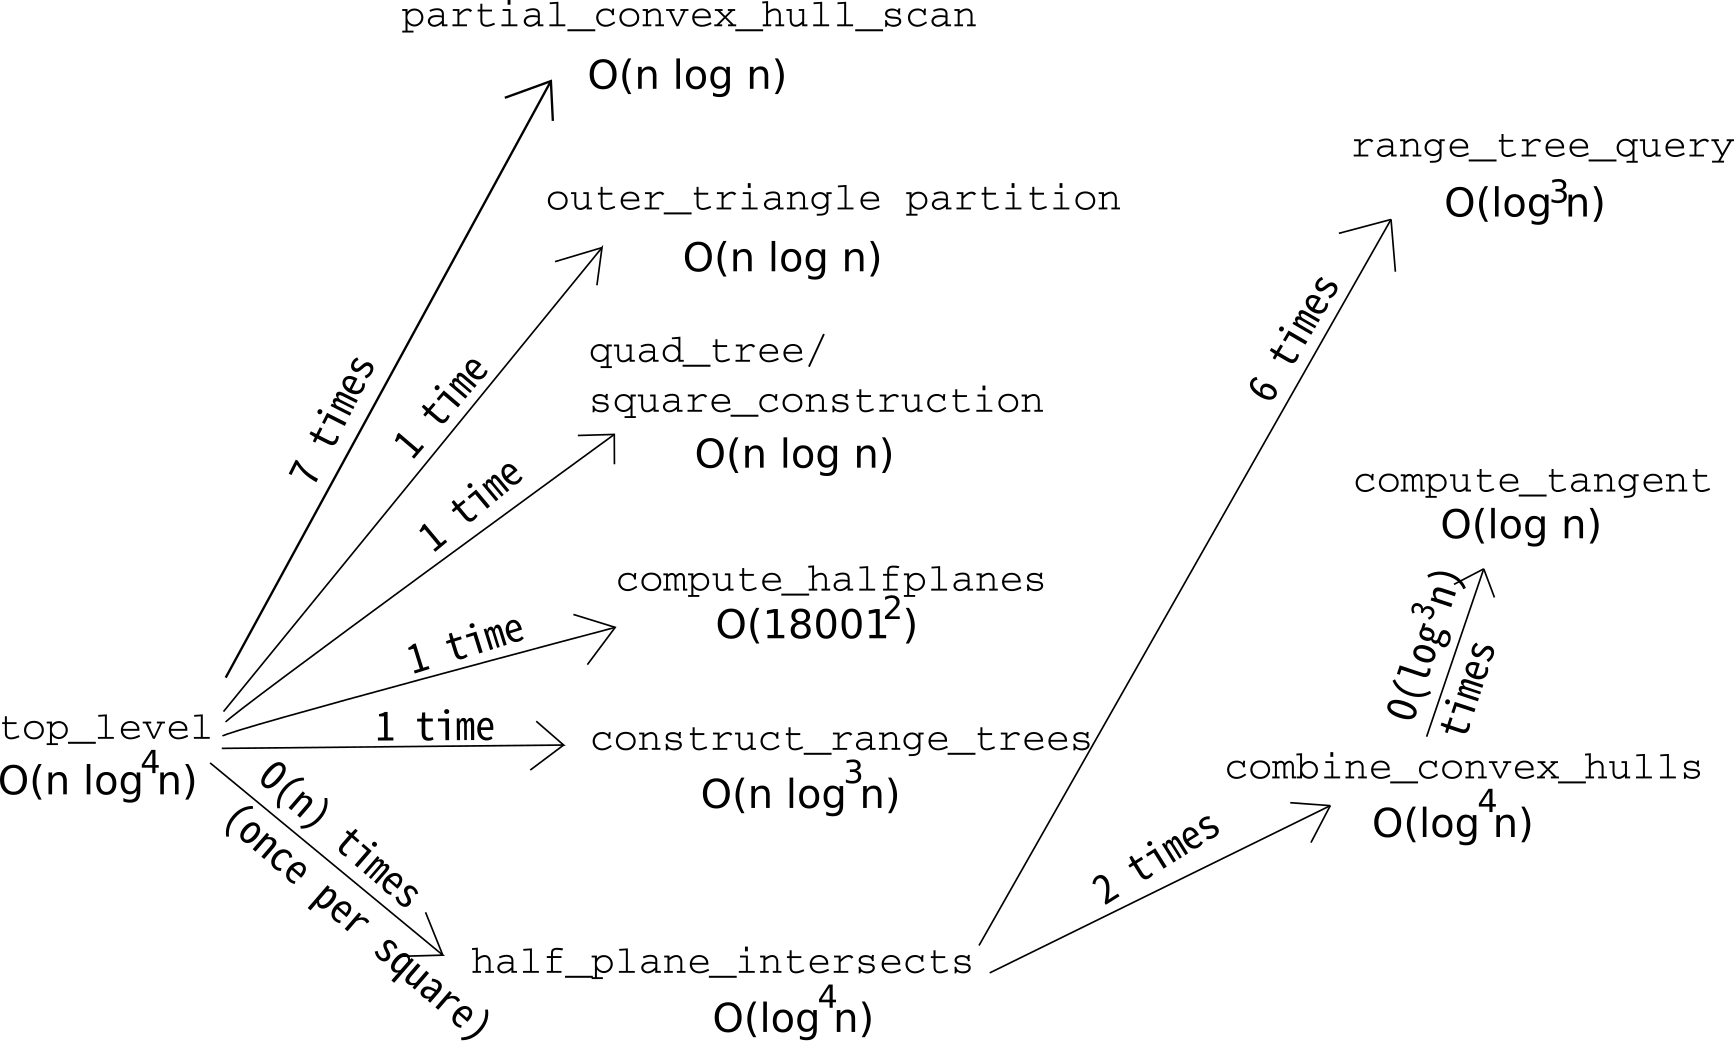
\includegraphics[width=0.75\textwidth]{hierarchy.png}
    \caption{Structural hierarchy of subroutines}
    \label{fig:hierarchy}
\end{figure}

The structural hierarchy of the subroutines for this algorithm is outlined in \figref{fig:hierarchy}.

\subsubsection{Partial Convex Hull Scan}

For a given angle $\phi$ and a set of points $P$, this subroutine computes the upper and lower halves of the convex hull of $P$, scanning through the nodes like in Graham's scan, but along a line with angle $\phi$ to the x-axis. This allows us to quickly compute convex hulls of a bipartition of $P$ separated by a line perpendicular to the scan direction. This operation takes $O(n \log n)$ time for a given angle, $n$ being the size of $P$.

\subsubsection{Outer Triangle Partition}

For a given set of points $P$, computes all triangles formed by three successive points on the set's convex hull, and finds and stores the subset of the points contained in each such triangle. This allows us to quickly compute the length of the convex hull of $P \ {p}$, where $p$ is a point on the convex hull of $P$. This operation takes $O(n \log n)$ time, where $n = |P|$.
    
\subsubsection{Quad Tree Construction} 

Each node in such a quad tree represents a square in the plane. Each node has four children, representing the regions of the four equal squares that make up their parent's region. The construction of a compressed quad tree over $n$ points takes $O(n \log n)$ time, given an appropriate computational model is used.

\subsubsection{Range Tree Construction and Search}

The range tree we construct here has three levels. The first level sorts the points on the x-axis, the subsequent level sorts the points at each node by the y-axis. The lowest level sort the points by a given direction in the plane. This allows us to easily find points that are restricted to a given rectangular axis-aligned region in the plane, and that are also inside a specified half-plane. This range tree also compute the convex hull of each node in the lowest level of the range tree. The range tree construction takes $O(n\log^3n)$, $n$ being the number of points over which we construct the tree.

\subsubsection{Tangent Computation} \label{subsub:Tangent}

For two polygons $A$ and $B$, computes their tangents using the algorithm provided in \cite{ks95}. We use this to determine which polygons belongs to the hull in the \textit{convex hull combining} subroutine. The algorithm uses $O(\log(a + b))$ time, where $a$ and $b$ are the number of points on the boundary of $A$ and $B$ respectively.

\subsubsection{Convex Hull Combining}
For a given set of convex hulls $\mathcal{C}$, finds the convex hull of all points on all the hulls. We use this to combine the convex hulls found from a query in the range tree described above, including its length, so that we can evaluate the perimeter. The running time for this subroutine is $O(k \log m)$, $k$ being the number of convex polygons, and $m$ the number of points on the hulls in total.

\section{Performance and Input Design}

% Performance analysis of each subroutine, as well as the entire algorithm. The sample input of the performance analysis could be from uniform sampling of the target rectangular region.

\subsection{Runtime Testing}

We primarily investigate how the runtime of each subroutine scales with respect to the size of input. The detailed hardware specifications and testing methodology are listed in \apdxref{apdxSpecs}.

\subsubsection{Tangent Computation}

The tangent computation, as described in \ref{subsub:Tangent}, is an $O(\log(a + b))$ subroutine, where $a$ and $b$ are the sizes of each polygon respectively. The tangent computation subroutine is tested on polygons of size $2^k$ for each $k \in [0, 15]$. For each $k$, the two polygons of size $2^k$ are independently generated by taking $2^k$ random samples of the unit circle under uniform distribution. For each size, the timing statistics are obtained by averaging $10^3$ such samples. The results are presented in  

\subsection{Designing Adversarial Inputs}

% Leverage the O(n log(n)) / O(n log^4(n)) distinction
In this section, we aim to identify the characteristics of ``adversarial inputs'', that is, inputs that impose a worst-case scenario on one or more subroutines of the algorithm. In the theoretical analysis by Abrahamsem et al. \cite{abb17}, $O(\log^4 n)$ runtime bound is given as a function of the input size $n$. Given a fixed $n$, the runtime bound does not include any characterization of the distribution of the set of input points. Nonetheless, observe that in the tangent computation subroutine, the runtime is a function of the sizes of each polygon, rather than the number of points contained within each polygon. Therefore, it is necessary for us to investigate how the distribution of points within a point set impacts the performance of the tangent computation subroutine, as well as the entire algorithm.

To be concrete, given a process of generating a point set $P$, we are interested in the expected complexity of $\CH(P)$. We first formalize the process of generating a point set. Given a bounded convex set $\mathcal{R} \subset \mathbb{R}^2$, as well as the number of points $n$. A point set $P_\mathcal{R}^D$ is generated via $n$ independent random samples of $\mathcal{R}$ under distribution $D$. Let $h_\mathcal{R}(n)^D$ denote the expected size of $\CH(P)$. Efron \cite{efr65} showed that if the expected area of $\CH(P)$ is at least $(1-f(n)) \mathrm{Area}(\mathcal{R})$, where $1 \geq f(n) \geq 0$ for $n \geq 0$, then the expected size of $\CH(P)$ is at most $nf(n/2)$ under uniform distribution. Based on this result, Har-Peled \cite{hp11} showed that if $\mathcal{R}$ resembles a convex polygon with $k$ sides, then $h_\mathcal{R}^U = O(k \log n)$, where $U$ denotes a uniform distribution over $\mathcal{R}$. And if $\mathcal{R}$ resembles a disk, then $h_\mathcal{R}^U = O(n^{1/3})$. On a more practical note, Raynaud \cite{ray70}, via integral estimation, showed that under $D \equiv N$ a normal distribution over $\mathcal{R}$, $h_\mathcal{R}^N = O((\log(n)^{1/2})$. Based on these findings, we will attempt to design a worst-case input for a fixed point-set size $n$ selected via independent uniform samples over a convex region. We will then compare this result with the point set selected under normal distribution. For completeness, we will also include the extreme case, where all points lie on the convex hull of the point set.

\subsubsection{Uniform Random Sampling on a Disk}



\subsection{Input Generation via Gradient Descent}

% Experimental input generation

\section{Implementation Difficulties}

After working with this algorithm, we have identified a couple of key issues concerning the practical use of the algorithm.

\textbf{RAM Usage} As we described, the algorithm requires us (at least if we wish to withhold the running time) to build and keep about $18000^2$ range trees in memories, one for each pair of 18001 points, each such tree of size $O(n log^3 n)$. An optimization that minimizes this number a little, is to exploit that many of the lines will be parallel: Since the range trees computed over the lines only depend on the angles of the lines, we can avoid many duplicate trees by pruning the ones corresponding to equal angles. A simple computation (see \texttt{/count\_unique\_line\_orientations} in \cite{hm18}) showed that the number of remaining unique line orientations was 63,431,423, which still imposes a huge memory consumption for large $n$.
\\ \
\textbf{The Convex Hull Combination Procedure} As mentioned before, we use a subroutine taking in $k$ convex hulls consisting of $m$ points in total. The paper claims that this subroutine runs in $O(k \log m)$ time. Our implementation of the routine, however, uses $O(m + k\log m)$ time, which shifts the total running time of the algorithm from $O(n \log^4 n)$ to $O(n^2)$ in the worst case.

The main problem is that our implementation computes each vertically sliced polygons explicitly, which automatically ramps up the running time to $O(m)$. We have failed to identify a proper way of implicitly storing these new polygons in a way that is suitable for the subsequent tangent computation we desire. 
\section{Conclusion}

\bibliographystyle{acm}
\bibliography{main}

\begin{appendices}
    \section{Hardware Specifications and Testing Methodology} \label{apdxSpecs}
\end{appendices}

\end{document}
